\documentclass[11pt]{article}

\usepackage[margin=1in]{geometry}
\usepackage{amsmath,amssymb,amsthm,mathtools,bm}
\usepackage{booktabs,tabularx,array,multirow}
\usepackage{graphicx}
\usepackage{subcaption}
\usepackage{enumitem}
\usepackage{algorithm}
\usepackage{algpseudocode}
\usepackage{xspace}
\usepackage{placeins}
\usepackage[numbers,sort&compress]{natbib}
\usepackage{xcolor}
\usepackage{microtype}
\usepackage[colorlinks=true,linkcolor=blue,citecolor=blue,urlcolor=blue]{hyperref}
\usepackage[nameinlink,capitalize]{cleveref}

\graphicspath{{figures/}}

\newtheorem{theorem}{Theorem}[section]
\newtheorem{lemma}[theorem]{Lemma}
\newtheorem{proposition}[theorem]{Proposition}
\newtheorem{corollary}[theorem]{Corollary}
\newtheorem{definition}[theorem]{Definition}
\newtheorem{assumption}[theorem]{Assumption}
\newtheorem{condition}[theorem]{Condition}
\newtheorem{example}[theorem]{Example}
\newtheorem{remark}[theorem]{Remark}

\newcommand{\E}{\mathbb E}
\newcommand{\Pp}{\mathbb P}
\newcommand{\R}{\mathbb R}
\newcommand{\N}{\mathbb N}
\newcommand{\Var}{\operatorname{Var}}
\newcommand{\Cov}{\operatorname{Cov}}
\newcommand{\1}{\mathbf 1}
\newcommand{\op}{\mathrm{op}}
\newcommand{\diag}{\operatorname{diag}}
\newcommand{\tr}{\operatorname{tr}}
\newcommand{\argmin}{\operatorname*{arg\,min}}
\newcommand{\argmax}{\operatorname*{arg\,max}}
\newcommand{\dist}{\operatorname{dist}}
\newcommand{\diam}{\operatorname{diam}}
\newcommand{\supp}{\operatorname{supp}}
\newcommand{\sgn}{\operatorname{sgn}}
\DeclarePairedDelimiter{\abs}{\lvert}{\rvert}
\DeclarePairedDelimiter{\norm}{\lVert}{\rVert}
\DeclarePairedDelimiter{\ip}{\langle}{\rangle}

\newcommand{\cA}{\mathcal A}
\newcommand{\cB}{\mathcal B}
\newcommand{\cD}{\mathcal D}
\newcommand{\cE}{\mathcal E}
\newcommand{\cF}{\mathcal F}
\newcommand{\cG}{\mathcal G}
\newcommand{\cH}{\mathcal H}
\newcommand{\cL}{\mathcal L}
\newcommand{\cM}{\mathcal M}
\newcommand{\cP}{\mathcal P}
\newcommand{\cS}{\mathcal S}
\newcommand{\cT}{\mathcal T}
\newcommand{\ThetaSet}{\Theta}
\newcommand{\DeltaN}{\Delta_N}
\newcommand{\CPT}{\ensuremath{\mathrm{CPT}}\xspace}
\newcommand{\CPTPG}{\ensuremath{\mathrm{CPT\mbox{-}PG}}\xspace}
\newcommand{\DRCPTPG}{\ensuremath{\mathrm{DRCPT\mbox{-}PG}}\xspace}
\newcommand{\EUPG}{\ensuremath{\mathrm{EU\mbox{-}PG}}\xspace}
\newcommand{\Dir}{\operatorname{Dirichlet}}
\newcommand{\Reg}{\mathcal R}
\newcommand{\Sta}{\mathsf S}
\newcommand{\eps}{\varepsilon}
\newcommand{\etaP}{\eta_{+}}
\newcommand{\etaM}{\eta_{-}}
\newcommand{\dH}{d_{\mathrm H}}
\newcommand{\db}{\mathrm{db}}
\newcommand{\pl}{\mathrm{pl}}
\newcommand{\cf}{\mathrm{cf}}
\newcommand{\as}{\mathrm{as}}

\title{Dynamic-Reference Cumulative Prospect Policy Gradients:\\Debiased Estimation, Minimax Limits, and Online Portfolio Tracking}
\author{Anonymous Authors}
\date{}

\begin{document}
\maketitle

\begin{abstract}
Cumulative prospect theory has become a principled route to reinforcement-learning agents whose risk attitudes resemble human decision makers.  Existing 
\CPT policy-gradient theory, however, is predominantly static: the environment is stationary and the psychological reference point is fixed.  This paper develops \emph{Dynamic-Reference Cumulative Prospect Policy Gradient} (\DRCPTPG), an online finite-horizon policy-gradient framework for portfolio learning in which the reference point evolves endogenously along the realized wealth path.  The framework combines an asymmetric path-dependent reference update, a regularized trajectory-level \CPT objective, a factor-parametrized Dirichlet policy on the portfolio simplex, and a debiased \CPT gradient estimator.  The theory gives a complete statistical layer for the estimator: the naive rank plug-in estimator is biased; a multilevel debiased estimator is exactly unbiased for the regularized \CPT gradient, has a finite-sample variance bound of order $M^{-1}$, obeys a multivariate central limit theorem, and attains the minimax $d/M$ gradient-estimation rate up to constants.  The optimization layer proves a dynamic-local-regret theorem,
\[
 {1\over K}\E \Reg_{\rho,w}(K)
 \le {C_0\over K\gamma}+C_1\gamma
 +{C_2\over K}\sum_{k=1}^{K}{1\over M_k}
 +{C_3\over K}\sum_{k=1}^{K}\delta_k^2
 +{C_4\over K}\sum_{k=1}^{K}\{\delta_k+\abs{r_{k+1}-r_k}\},
\]
which separates the costs of optimization, finite-sample \CPT estimation, exogenous market drift, and endogenous reference drift.  Theory-aligned experiments on a semi-synthetic A-share-style market and heterogeneous retail-agent evaluation show the predicted path dependence, disposition-effect amplification, post-shock tracking advantage over static-reference baselines, and the practical meaning of the estimator theory.
\end{abstract}

\paragraph{One-sentence contribution.}
This paper turns the psychological reference point from a fixed hyperparameter into an endogenous state variable in \CPT policy optimization, then supplies the estimator theory and dynamic-regret analysis needed to learn against the resulting moving nonconvex target.

\section{Introduction}\label{sec:introduction}

Reinforcement learning is a general computational language for sequential decision making: an agent observes a state, chooses an action, receives feedback, and updates its policy.  This paradigm has been powerful in engineering control, games, and online recommendation.  In human-facing domains, however, the usual expected-return objective is often the wrong behavioral target.  A robo-advisor who maximizes expected wealth may recommend a portfolio that is statistically efficient but psychologically unacceptable after a drawdown; a trading assistant that ignores a user's reference point may generate advice that is rejected even when it improves objective return.  The issue is not merely risk aversion.  Human decision makers evaluate uncertain outcomes through reference dependence, loss aversion, and nonlinear probability weighting.

Cumulative prospect theory (\CPT) formalizes these features through a rank-dependent functional of the whole outcome distribution \citep{kahneman1979prospect,tversky1992advances}.  This has motivated \CPT-RL methods that optimize prospect-theoretic returns instead of expected returns \citep{prashanth2016cumulative,jie2018stochastic,ramasubramanian2021reinforcement,lepel2024policygradients}.  The methodological shift is substantial: \CPT is not a one-step reward transformation, not a mean-variance penalty, and not an ordinary concave utility.  It is a generally nonconvex functional of the trajectory-level return distribution, with different treatments of gains and losses.

This paper focuses on a structural gap in this line of work.  Existing \CPT-RL theory usually treats the reference point as a fixed constant.  Behavioral and mathematical-finance evidence points in the opposite direction: reference points adapt after gains and losses, and the adaptation can be asymmetric \citep{arkes2008reference,arkes2010cross,he2019realization,qin2022realization}.  Consider the simplest investment story.  An investor starts with wealth $1.0$, first rises to $1.4$, and then falls to $1.2$.  Another investor starts at $1.0$, first falls to $0.8$, and then recovers to $1.2$.  The two paths have the same terminal wealth, but the first path is plausibly experienced as a loss from a recently raised benchmark, while the second is experienced as a gain from a depressed benchmark.  A fixed-reference \CPT agent treats these two terminal outcomes as equivalent; a dynamic-reference agent does not.

The failure has both theoretical and practical consequences.  Once the reference point moves along the path, the policy optimization problem becomes doubly nonstationary.  Market regimes, volatility, and factor returns generate exogenous drift.  At the same time, the agent's portfolio changes wealth, wealth changes the reference point, and the reference point changes the next \CPT objective.  The target first-order stationary set is therefore moving because the world changes and because the agent's own actions move the user's psychological state.  A proof of convergence to a fixed stationary point no longer answers the right question.  The right question is whether the algorithm can \emph{track} the moving \CPT target and how much of the tracking error is due to sampling, market drift, and reference drift.

We answer this question through \DRCPTPG.  The model is designed for an online portfolio-advice scenario: a retail investor starts with normalized wealth, allocates among several risky assets and cash, receives recommendations over short horizons, and updates a psychological benchmark after each realized wealth change.  The policy is a Dirichlet distribution whose concentration parameters are exponential functions of interpretable asset factors.  This avoids directly learning unconstrained high-dimensional portfolio weights and enforces the simplex constraint by construction.  Each episode has two layers.  The execution layer uses the current policy mean to recommend a stable portfolio and update the real reference point.  The learning layer resimulates horizon-$h$ trajectories from the same episode-start state, computes trajectory-level \CPT ranks, and updates the policy parameter by a debiased \CPT gradient estimate.

The most delicate part is estimation.  \CPT gradients depend on the derivative of a probability-weighting function evaluated at the unknown survival distribution of the outcome.  A rank plug-in estimator is natural but biased because the probability-weighting derivative is nonlinear.  We therefore first analyze the bias and then remove it.  The paper introduces a multilevel debiased estimator, in the spirit of randomized telescoping estimators \citep{rhee2015unbiased}, that is exactly unbiased for the regularized \CPT gradient.  It has finite variance, obeys a central limit theorem, and achieves the minimax $d/M$ gradient-estimation rate.  This estimator layer feeds directly into the dynamic local regret bound.

The resulting insight is counterintuitive but useful.  Reference adaptation improves behavioral alignment only by making the target move.  A more adaptive reference can therefore reduce behavioral misspecification while increasing the statistical tracking budget.  The theorem makes this trade-off explicit: the dynamic local regret contains separate terms for sample size, market drift, and reference drift.  Dynamic reference points are not noise to be averaged away; they are endogenous target drift to be measured and controlled.

\paragraph{Contributions.}
\begin{enumerate}[leftmargin=2em]
\item \textbf{Dynamic-reference \CPT-PG.}  We extend static-reference \CPT policy gradients to a nonstationary finite-horizon setting in which references evolve path by path.  Static \CPTPG is recovered as the special case $r_{k+1}=r_k$ and $\delta_k=0$.
\item \textbf{Estimator theory.}  We prove a \CPT score-gradient identity, show why the finite-rank plug-in estimator is biased, construct an exactly unbiased multilevel estimator, bound its finite-sample variance, prove asymptotic normality, and establish a minimax lower bound.
\item \textbf{Tracking theory.}  We prove path dependence, drift stability of moving stationary sets, a dynamic-local-regret upper bound, and a stationary-set tracking corollary under a local error-bound condition.
\item \textbf{Behavioral validation.}  Synthetic experiments test path dependence and disposition-effect amplification under asymmetric reference adaptation.
\item \textbf{Portfolio and retail-agent evidence.}  A semi-synthetic A-share-style market with five stocks plus cash evaluates post-shock tracking, ablations, and sensitivity; a heterogeneous retail-agent evaluation measures adoption and satisfaction across advisor baselines.
\end{enumerate}

\paragraph{Organization.}
\Cref{sec:related} positions the work.  \Cref{sec:setup} defines the dynamic-reference \CPT objective and assumptions.  \Cref{sec:algorithm} gives the Dirichlet policy and \DRCPTPG.  \Cref{sec:results} states the estimator, regret, asymptotic, and minimax results.  \Cref{sec:experiments} reports theorem-aligned evidence.  \Cref{sec:discussion} discusses scope and future research.  All proofs are in the appendix.

\section{Related Work and Positioning}\label{sec:related}

\paragraph{CPT and reinforcement learning.}
\citet{kahneman1979prospect,tversky1992advances} introduced prospect theory and cumulative prospect theory as alternatives to expected utility.  \citet{prashanth2016cumulative} brought \CPT into reinforcement learning and emphasized that \CPT evaluates a return distribution rather than an immediate reward.  \citet{jie2018stochastic} studied stochastic optimization under \CPT, while \citet{lepel2024policygradients} derived policy-gradient methods for cumulative prospect objectives.  Our work uses the policy-gradient viewpoint but replaces the fixed reference point by a path-dependent state variable.

\paragraph{Behavioral alignment beyond expectation.}
Risk-sensitive RL often uses variance penalties, coherent risk measures, or exponential utility.  \CPT is different because rank-dependent weighting and reference-dependent gains/losses can represent behaviors that standard risk-sensitive utilities cannot.  \citet{ramasubramanian2021reinforcement} argue that expectation alone is insufficient for agents designed to align with human preferences, and \citet{lalmohammed2025modeling} show that prospect-theoretic multi-agent policies can reproduce human-like strategic phenomena.  Our paper studies the optimization theory needed when the human evaluation state itself evolves over time.

\paragraph{Reference adaptation.}
\citet{arkes2008reference,arkes2010cross} document reference adaptation in trading-like experiments, including asymmetric adaptation after gains and losses.  \citet{he2019realization} show that adaptive references can strengthen the disposition effect, while \citet{qin2022realization} model path-dependent reference points.  These papers motivate the reference dynamics used here.  Our contribution is to integrate these dynamics into online \CPT policy-gradient learning and to provide estimator and regret guarantees.

\paragraph{Nonconvex online learning.}
Because \CPT objectives are nonconvex and time-varying, global regret against a fixed comparator is not the relevant performance criterion.  Dynamic local regret for nonconvex online problems measures whether recent gradients are small under a moving environment \citep{hazan2017efficient,aydore2019dynamic,hallak2021regret}.  We adapt this idea to a rank-dependent, path-dependent \CPT objective and add an endogenous reference-drift term.

\paragraph{Debiased and minimax estimation.}
The gradient-estimation difficulty comes from a nonlinear functional of an unknown outcome distribution.  Our multilevel debiasing argument follows the randomized telescoping principle of \citet{rhee2015unbiased}.  The asymptotic normality and minimax lower-bound proofs use standard empirical-process and decision-theoretic tools \citep{vandervaart1998asymptotic,tsybakov2009introduction}.

\paragraph{Portfolio learning.}
Classical portfolio theory optimizes mean-variance trade-offs \citep{markowitz1952portfolio}; factor models provide interpretable predictors for asset returns \citep{fama1993common}.  We keep factor interpretability but change the objective from expected or exponential utility to dynamic-reference \CPT.  The Dirichlet policy is used because it produces valid long-only portfolio weights without an additional projection step.

\section{Problem Setup}\label{sec:setup}

\subsection{Nonstationary episodic portfolio MDP}

Trading occurs in episodes $k=1,\ldots,K$.  Episode $k$ begins at date $t_k$ and lasts $h$ trading days.  At date $u\in\{t_k,\ldots,t_k+h-1\}$ the state is
\[
 s_u=(\text{market factors},\;X_u,\;r_u,\;\omega_{u-1}),
\]
where $X_u$ is normalized wealth, $r_u$ is the psychological reference point, and $\omega_{u-1}$ is the previous portfolio.  The action is a long-only portfolio
\[
 \omega_u=(\omega_{0,u},\omega_{1,u},\ldots,\omega_{N,u})\in \Delta_N
 :=\left\{\omega\in\R_+^{N+1}:\sum_{i=0}^{N}\omega_i=1\right\},
\]
with asset $0$ denoting cash.  Let $R_{u+1}\in\R^{N+1}$ be the next-period excess-return vector, with $R_{0,u+1}=0$ for cash.  With proportional transaction cost $c_{\rm tc}\ge0$,
\begin{equation}\label{eq:wealth-update}
 X_{u+1}=X_u\left(1+\omega_u^\top R_{u+1}-c_{\rm tc}\norm{\omega_u-\omega_{u-1}}_1\right),
 \qquad X_1=1.
\end{equation}
The transition law may change with $k$; this is the exogenous nonstationarity of the market.

\subsection{Asymmetric dynamic references}

The reference point is updated after each realized wealth observation by
\begin{equation}\label{eq:reference-update}
 r_{u+1}=\Phi(r_u,X_{u+1})=
 \begin{cases}
 r_u+\etaP(X_{u+1}-r_u), & X_{u+1}\ge r_u,\\[2pt]
 r_u-\etaM(r_u-X_{u+1}), & X_{u+1}<r_u,
 \end{cases}
\end{equation}
where $\etaP,\etaM\in[0,1]$.  The empirically motivated case is $\etaP>\etaM$: gains move the benchmark upward faster than losses move it downward.  A trajectory $\tau$ in episode $k$ generates terminal wealth $X_k(\tau)$ and terminal reference $r_{k,h}(\tau)$.  The relative outcome evaluated by \CPT is
\begin{equation}\label{eq:relative-outcome}
 Y_k(\tau)=X_k(\tau)-r_{k,h}(\tau).
\end{equation}

\subsection{Regularized cumulative-prospect objective}

Let $Y^+=\max\{Y,0\}$ and $Y^-=\max\{-Y,0\}$.  The gain and loss value functions are
\begin{equation}\label{eq:value-functions}
 v_+(Y)=(Y^+)^{\alpha_+},\qquad
 v_-(Y)=\lambda(Y^-)^{\alpha_-},
\end{equation}
where $\lambda>1$ and $\alpha_+,\alpha_-\in(0,1]$.  The probability weights are regularized Tversky-Kahneman weights
\begin{equation}\label{eq:prob-weights}
 w_\pm^\eps(p)=w_\pm(\eps+(1-2\eps)p),\qquad
 w_\pm(p)=\frac{p^{\beta_\pm}}{\{p^{\beta_\pm}+(1-p)^{\beta_\pm}\}^{1/\beta_\pm}},
\end{equation}
with $\eps\in(0,1/2)$.  We also smooth $y\mapsto (y^\pm)^{\alpha_\pm}$ inside $[-\eps,\eps]$ when $\alpha_\pm<1$ so that the objective is differentiable.

Let $\Pp_{k,\theta}$ be the horizon-$h$ trajectory law induced by policy $\pi_\theta$ from the episode-$k$ start state.  Define survival functions
\[
 S^+_{k,\theta}(z)=\Pp_{k,\theta}\{v_+(Y_k)>z\},\qquad
 S^-_{k,\theta}(z)=\Pp_{k,\theta}\{v_-(Y_k)>z\}.
\]
By boundedness below, it is enough to integrate over $[0,B_v]$ for a finite $B_v$.  The regularized dynamic-reference \CPT objective is
\begin{equation}\label{eq:cpt-objective}
 J_k(\theta,r_k)
 =\int_0^{B_v} w_+^\eps(S^+_{k,\theta}(z))\,dz
 -\int_0^{B_v} w_-^\eps(S^-_{k,\theta}(z))\,dz.
\end{equation}
This is a functional of the entire distribution of $Y_k$, not a sum of one-period rewards.

\subsection{Moving stationary sets and dynamic local regret}

The episode-$k$ first-order stationary set is
\begin{equation}\label{eq:stationary-set}
 \Sta_k=\{\theta\in\ThetaSet:\nabla_\theta J_k(\theta,r_k)=0\}.
\end{equation}
Because both the market law and $r_k$ evolve, $\Sta_k$ moves.  Let
\[
 g_k=\nabla_\theta J_k(\theta_k,r_k).
\]
For window length $w\ge1$ and discount $\rho\in(0,1]$, define
\begin{equation}\label{eq:smoothed-gradient}
 \bar g_k={1\over A_k}\sum_{j=0}^{\min\{w-1,k-1\}}\rho^j g_{k-j},
 \qquad
 A_k=\sum_{j=0}^{\min\{w-1,k-1\}}\rho^j.
\end{equation}
The dynamic local regret is
\begin{equation}\label{eq:dynamic-regret}
 \Reg_{\rho,w}(K)=\sum_{k=1}^{K}\norm{\bar g_k}_2^2.
\end{equation}
The criterion asks whether the recent gradients of the moving objectives are small.

\subsection{Assumptions, diagnostics, and fallback interpretations}\label{subsec:assumptions}

The assumptions are local to the compact domain visited by the algorithm.  Each has a statistical role, an empirical diagnostic, and a fallback interpretation.

\begin{assumption}[Bounded local domain]\label{ass:bounded}
There are constants $B_X,B_r,B_G,B_v<\infty$ such that, on the analyzed domain, $\abs{X_u}\le B_X$, $\abs{r_u}\le B_r$, $\abs{v_\pm(Y_k)}\le B_v$, and the score function
\[
 G_{k,\theta}(\tau)=\sum_{u=t_k}^{t_k+h-1}\nabla_\theta\log \pi_\theta(\omega_u\mid s_u)
\]
satisfies $\norm{G_{k,\theta}(\tau)}_2\le B_G$.
\end{assumption}
\emph{Role.}  Keeps \CPT weights and score products integrable.  \emph{Diagnostic.}  Report wealth range, drawdown, reference range, and score norms.  \emph{Fallback.}  State the theorem locally before leverage, ruin, or simplex-boundary events.

\begin{assumption}[Regularized smooth \CPT]\label{ass:smooth-cpt}
For fixed $\eps>0$, $w_\pm^\eps$ are twice continuously differentiable with bounded first and second derivatives on $[0,1]$, and $\theta\mapsto J_k(\theta,r_k)$ is $L$-smooth on compact convex $\ThetaSet$.
\end{assumption}
\emph{Role.}  Removes endpoint singularities in probability weighting and the kink at zero relative outcome.  \emph{Diagnostic.}  Report sensitivity to $\eps$ and the frequency of extreme rank probabilities.  \emph{Fallback.}  Interpret results as applying to the smoothed estimable \CPT objective.

\begin{assumption}[Market and reference drift]\label{ass:drift}
There exists a drift budget $\delta_k\ge0$ such that the horizon-$h$ trajectory laws in adjacent episodes are within $\delta_k$ in bounded-Lipschitz distance, uniformly over $\theta\in\ThetaSet$.  Moreover, for all $\theta\in\ThetaSet$,
\begin{align}
 \norm{\nabla J_{k+1}(\theta,r_{k+1})-\nabla J_k(\theta,r_k)}_2
 &\le L_D\{\delta_k+\abs{r_{k+1}-r_k}\},\label{eq:gradient-drift}\\
 \abs{J_{k+1}(\theta,r_{k+1})-J_k(\theta,r_k)}
 &\le L_J\{\delta_k+\abs{r_{k+1}-r_k}\}.
 \label{eq:value-drift}
\end{align}
\end{assumption}
\emph{Role.}  Quantifies the two sources of nonstationarity.  \emph{Diagnostic.}  Rolling means, volatility shifts, factor covariance shifts, and reference increments.  \emph{Fallback.}  Large structural breaks enlarge the bound or trigger a reset.

\begin{assumption}[Multilevel regularity of the CPT multiplier]\label{ass:mlmc}
Let $T_{k,\ell}$ be the coupled cross-fitted rank estimator of $g_k$ using $N_0 2^\ell$ quantile trajectories and a fixed score replication, and let $\mu_{k,\ell}=\E(T_{k,\ell}\mid\cF_k)$.  There exists $A_{\rm ml}<\infty$ such that
\[
 \norm{\mu_{k,\ell}-g_k}_2\le A_{\rm ml}2^{-\ell},\qquad
 \E\norm{T_{k,\ell}-{1\over2}(T_{k,\ell-1}^{(1)}+T_{k,\ell-1}^{(2)})}_2^2\le A_{\rm ml}2^{-2\ell},
\]
where $T_{k,\ell-1}^{(1)}$ and $T_{k,\ell-1}^{(2)}$ are the two half-sample estimators coupled inside $T_{k,\ell}$.
\end{assumption}
\emph{Role.}  Ensures that randomized telescoping produces an unbiased finite-variance estimator.  \emph{Diagnostic.}  Plot plug-in bias and level-difference variance against $2^{-\ell}$.  \emph{Fallback.}  Use a truncated debiased estimator and include its residual bias term.

\begin{assumption}[Normalized update alignment]\label{ass:alignment}
The implemented direction $d_k=d(\widehat g_k^{\db})$ satisfies $\norm{d_k}_2\le D_d$ and
\begin{equation}\label{eq:alignment}
 \E[\ip{g_k,d_k}\mid\cF_k]
 \ge c_d\norm{g_k}_2^2-c_e\E[\norm{\widehat g_k^{\db}-g_k}_2^2\mid\cF_k]
\end{equation}
for constants $c_d>0$ and $c_e\ge0$.
\end{assumption}
\emph{Role.}  Converts a noisy normalized update into expected ascent.  \emph{Diagnostic.}  Cosine similarity between two independent gradient estimates.  \emph{Fallback.}  Use ordinary projected stochastic gradient ascent, for which the same proof is simpler.

\begin{assumption}[Stationary-set error bound]\label{ass:error-bound}
Each $\Sta_k$ is nonempty and closed, and for some $\kappa<\infty$,
\begin{equation}\label{eq:error-bound}
 \dist(\theta,\Sta_k)\le \kappa\norm{\nabla J_k(\theta,r_k)}_2,
 \qquad \theta\in\ThetaSet.
\end{equation}
\end{assumption}
\emph{Role.}  Converts small gradient into distance to the moving stationary set.  \emph{Diagnostic.}  Multi-start local search and empirical gradient-distance calibration.  \emph{Fallback.}  Without this condition, the regret theorem remains a squared-gradient guarantee.

\section{Algorithm}\label{sec:algorithm}

\subsection{Dirichlet policy on the portfolio simplex}

For asset $i\in\{0,\ldots,N\}$ at date $u$, let $q_{i,u}\in\R^d$ be a bounded feature vector containing momentum, reversal, volatility, value, a cash indicator, and previous-position information.  The policy parameter $\theta\in\R^d$ assigns scores
\begin{equation}\label{eq:dir-score}
 z_{i,u}=\theta^\top q_{i,u},\qquad a_{i,u}=\exp(z_{i,u}),
\end{equation}
and samples
\begin{equation}\label{eq:dirichlet-policy}
 \omega_u\sim\pi_\theta(\cdot\mid s_u)=\Dir(a_{0,u},\ldots,a_{N,u}).
\end{equation}
For the real recommendation, the policy mean
\begin{equation}\label{eq:dirichlet-mean}
 \bar\omega_{i,u}={a_{i,u}\over\sum_{j=0}^{N}a_{j,u}}
\end{equation}
is used to avoid excessive turnover.  The stochastic policy is used in the learning layer to estimate the \CPT gradient.

\begin{algorithm}[t]
\caption{Dirichlet factor policy for portfolio generation}\label{alg:dirichlet}
\begin{algorithmic}[1]
\Require State $s_u$, previous portfolio $\omega_{u-1}$, factors $q_{i,u}$, parameter $\theta$, execution mode $e\in\{\mathrm{sample},\mathrm{mean}\}$.
\For{$i=0,\ldots,N$}
    \State Compute $z_{i,u}=\theta^\top q_{i,u}$ and concentration $a_{i,u}=\exp(z_{i,u})$.
\EndFor
\If{$e=\mathrm{sample}$}
    \State Draw $\omega_u\sim\Dir(a_{0,u},\ldots,a_{N,u})$.
\Else
    \State Set $\omega_{i,u}=a_{i,u}/\sum_{j=0}^{N}a_{j,u}$.
\EndIf
\State \Return $\omega_u\in\Delta_N$.
\end{algorithmic}
\end{algorithm}

\subsection{Debiased CPT policy-gradient update}

The algorithm separates execution from learning.  The execution path is the single portfolio path recommended to the investor.  The learning paths are Monte Carlo trajectories from the same episode-start state.

\begin{algorithm}[t]
\caption{Dynamic-reference \CPT policy gradient (\DRCPTPG)}\label{alg:drcptpg}
\begin{algorithmic}[1]
\Require Initial parameter $\theta_1$, initial wealth $X_1=1$, initial reference $r_1$, horizon $h$, step size $\gamma$, \CPT parameters $(\lambda,\alpha_\pm,\beta_\pm,\eps)$, reference rates $(\etaP,\etaM)$, debiased replications $M_k$.
\State Initialize previous portfolio $\omega_0=(1,0,\ldots,0)$.
\For{$k=1,2,\ldots,K$}
    \State Record episode-start state $(s_{t_k},\omega_{t_k-1},X_{t_k},r_k,\theta_k)$.
    \State \textbf{Execution layer:} for $u=t_k,\ldots,t_k+h-1$, use Algorithm \ref{alg:dirichlet} with $e=\mathrm{mean}$, update wealth by \eqref{eq:wealth-update}, and update reference by \eqref{eq:reference-update}.
    \State Set $r_{k+1}=r_{t_k+h}$.
    \State \textbf{Learning layer:} from the same episode-start state, construct $M_k$ independent multilevel debiased \CPT gradient replications $Z_{k,1}^{\db},\ldots,Z_{k,M_k}^{\db}$ by Algorithm \ref{alg:debiased}.
    \State Set $\widehat g_k^{\db}=M_k^{-1}\sum_{b=1}^{M_k} Z_{k,b}^{\db}$.
    \State Normalize $d_k=\widehat g_k^{\db}/\max\{\norm{\widehat g_k^{\db}}_2,a_0\}$ for a small fixed $a_0>0$.
    \State Update $\theta_{k+1}=\Pi_{\ThetaSet}(\theta_k+\gamma d_k)$.
\EndFor
\State \Return portfolios, wealth path, reference path, parameters, and diagnostics.
\end{algorithmic}
\end{algorithm}

\begin{algorithm}[t]
\caption{One multilevel debiased \CPT gradient replication}\label{alg:debiased}
\begin{algorithmic}[1]
\Require Episode-start state, parameter $\theta_k$, base level $N_0$, level probabilities $p_\ell\propto2^{-a\ell}$ with $a\in(1,2)$.
\State Draw a random level $L\in\{0,1,2,\ldots\}$ with $\Pp(L=\ell)=p_\ell$.
\If{$L=0$}
    \State Generate the cross-fitted rank estimator $T_{k,0}$ and set $\Delta_{k,0}=T_{k,0}$.
\Else
    \State Generate a coupled estimator $T_{k,L}$ using $N_0 2^L$ quantile trajectories and its two half-sample estimators $T_{k,L-1}^{(1)}$, $T_{k,L-1}^{(2)}$.
    \State Set $\Delta_{k,L}=T_{k,L}-{1\over2}(T_{k,L-1}^{(1)}+T_{k,L-1}^{(2)})$.
\EndIf
\State \Return $Z_{k}^{\db}=\Delta_{k,L}/p_L$.
\end{algorithmic}
\end{algorithm}

\section{Main Results}\label{sec:results}

\subsection{Dynamic reference creates genuine path dependence}

\begin{proposition}[Same terminal wealth, different \CPT input]\label{prop:path-dependence}
Let $L<r_0<C<H$.  Consider two two-step wealth paths with common initial reference $r_0$ and common terminal wealth $C$:
\[
 A: r_0\to H\to C,
 \qquad
 B: r_0\to L\to C.
\]
Under the reference update \eqref{eq:reference-update}, assume $C< (1-\etaP)r_0+\etaP H$ and $C>(1-\etaM)r_0+\etaM L$, so the second step is a loss for path $A$ and a gain for path $B$.  The terminal references satisfy
\begin{equation}\label{eq:path-diff}
 r_A-r_B=\etaP(1-\etaM)H-\etaM(1-\etaP)L+(\etaM-\etaP)C.
\end{equation}
Whenever this quantity is nonzero, the two paths have different relative outcomes $C-r_A$ and $C-r_B$ and hence different regularized \CPT values.
\end{proposition}

\subsection{CPT score-gradient identity}

\begin{theorem}[Regularized \CPT policy-gradient identity]\label{thm:gradient-identity}
Suppose Assumptions \ref{ass:bounded} and \ref{ass:smooth-cpt} hold and the trajectory law is differentiable in quadratic mean with score $G_{k,\theta}$.  Define
\begin{align}\label{eq:psi-def}
 \psi_{k,\theta}(\tau)
 =&\int_0^{B_v}\dot w_+^\eps(S^+_{k,\theta}(z))
 \{\1[v_+(Y_k(\tau))>z]-S^+_{k,\theta}(z)\}\,dz\notag\\
 &-\int_0^{B_v}\dot w_-^\eps(S^-_{k,\theta}(z))
 \{\1[v_-(Y_k(\tau))>z]-S^-_{k,\theta}(z)\}\,dz.
\end{align}
Then
\begin{equation}\label{eq:gradient-identity}
 \nabla_\theta J_k(\theta,r_k)=
 \E_{k,\theta}\{\psi_{k,\theta}(\tau)G_{k,\theta}(\tau)\}.
\end{equation}
Consequently, if $\psi_{k,\theta}$ were known, the oracle estimator $m^{-1}\sum_{j=1}^{m}\psi_{k,\theta}(\tau_j)G_{k,\theta}(\tau_j)$ would be unbiased.
\end{theorem}

\paragraph{Why a debiasing step is needed.}
The multiplier \eqref{eq:psi-def} contains the unknown survival functions $S^\pm_{k,\theta}$.  Replacing them by empirical ranks gives a convenient plug-in estimator, but it is not exactly unbiased because $\dot w_\pm^\eps(\cdot)$ is nonlinear.  The next result quantifies the bias and then removes it.

\begin{proposition}[Plug-in bias and debiased estimator]\label{prop:debias}
Let $\widehat g_{k,n,m}^{\pl}$ be the cross-fitted rank plug-in estimator using $n$ trajectories for survival estimation and $m$ independent trajectories for score averaging.  Under Assumptions \ref{ass:bounded} and \ref{ass:smooth-cpt},
\begin{equation}\label{eq:plugin-bias}
 \norm{\E(\widehat g_{k,n,m}^{\pl}\mid\cF_k)-g_k}_2\le {C_{\rm b}\over n}+C_{\rm d}\delta_k.
\end{equation}
Under Assumption \ref{ass:mlmc}, Algorithm \ref{alg:debiased} produces a random vector $Z_k^{\db}$ such that
\begin{equation}\label{eq:db-unbiased}
 \E(Z_k^{\db}\mid\cF_k)=g_k.
\end{equation}
Moreover, with $p_\ell\propto2^{-a\ell}$ and $a\in(1,2)$,
\begin{equation}\label{eq:db-second-moment}
 \E\norm{Z_k^{\db}}_2^2\le C_{\db}<\infty,
 \qquad
 \E[\mathrm{cost}(Z_k^{\db})]<\infty.
\end{equation}
If the telescoping sum is truncated at level $L_{\max}$, the residual bias is bounded by $A_{\rm ml}2^{-L_{\max}}$.
\end{proposition}

\subsection{Finite-sample variance and asymptotic distribution}

\begin{theorem}[Finite-sample variance bound]\label{thm:variance}
Let
\[
 \widehat g_{k,M}^{\db}={1\over M}\sum_{b=1}^{M}Z_{k,b}^{\db},
\]
where the $Z_{k,b}^{\db}$ are independent copies of Algorithm \ref{alg:debiased}.  Under Assumption \ref{ass:mlmc},
\begin{equation}\label{eq:variance-bound}
 \E(\widehat g_{k,M}^{\db}\mid\cF_k)=g_k,
 \qquad
 \tr\Var(\widehat g_{k,M}^{\db}\mid\cF_k)
 \le {C_{\db}\over M}.
\end{equation}
For the practical plug-in estimator,
\begin{equation}\label{eq:plugin-mse}
 \E\norm{\widehat g_{k,n,m}^{\pl}-g_k}_2^2
 \le {C_n\over n}+{C_m\over m}+C_\delta\delta_k^2+{C_{\rm b}^2\over n^2}.
\end{equation}
\end{theorem}

\begin{theorem}[Asymptotic normality of the debiased gradient estimator]\label{thm:clt}
Suppose $Z_k^{\db}$ has a conditional $(2+\xi)$ moment for some $\xi>0$, and let
\[
 \Sigma_k=\Var(Z_k^{\db}\mid\cF_k)
\]
be nonsingular.  Conditional on $\cF_k$,
\begin{equation}\label{eq:clt}
 \sqrt{M}\,\Sigma_k^{-1/2}(\widehat g_{k,M}^{\db}-g_k)
 \rightsquigarrow N(0,I_d).
\end{equation}
If $\widehat\Sigma_k$ is the empirical covariance of the $M$ debiased replications and $d$ is fixed, then the studentized statistic obtained by replacing $\Sigma_k$ by $\widehat\Sigma_k$ also converges to $N(0,I_d)$.
\end{theorem}

\subsection{Dynamic local regret}

\begin{lemma}[Drift of stationary sets]\label{lem:set-drift}
Under Assumptions \ref{ass:drift} and \ref{ass:error-bound},
\begin{equation}\label{eq:set-drift}
 \dH(\Sta_{k+1},\Sta_k)
 \le \kappa L_D\{\delta_k+\abs{r_{k+1}-r_k}\}.
\end{equation}
\end{lemma}

\begin{theorem}[Dynamic local regret of \DRCPTPG]\label{thm:dynamic-regret}
Suppose Assumptions \ref{ass:bounded}--\ref{ass:alignment} hold.  Algorithm \ref{alg:drcptpg} uses $M_k$ debiased gradient replications and a fixed step size $\gamma>0$.  Then there exist finite constants $C_0,\ldots,C_4$, independent of $K$ and $M_k$, such that
\begin{equation}\label{eq:main-bound}
 {1\over K}\E\Reg_{\rho,w}(K)
 \le {C_0\over K\gamma}+C_1\gamma
 +{C_2\over K}\sum_{k=1}^{K}{1\over M_k}
 +{C_3\over K}\sum_{k=1}^{K}\delta_k^2
 +{C_4\over K}\sum_{k=1}^{K}\{\delta_k+\abs{r_{k+1}-r_k}\}.
\end{equation}
If a truncated debiased estimator with level $L_{k,\max}$ is used, the right-hand side gains the additional term
\[
 {C_5\over K}\sum_{k=1}^{K}2^{-2L_{k,\max}}.
\]
\end{theorem}

\paragraph{Interpretation.}
The result is a tracking theorem.  It does not claim global optimality or monotone wealth improvement.  It says that the average squared gradient of the moving \CPT objective is controlled by five interpretable budgets: optimization, estimator variance, market drift, reference drift, and truncation bias if exact debiasing is not used.

\begin{corollary}[Static-reference limit]\label{cor:static}
If the market is stationary, $\delta_k=0$, the reference is fixed, $r_{k+1}=r_k=r$, and $M_k\to\infty$, then \DRCPTPG reduces to static-reference \CPTPG and
\begin{equation}\label{eq:static-corollary}
 \limsup_{K\to\infty}{1\over K}\sum_{k=1}^{K}\E\norm{\nabla J(\theta_k,r)}_2^2\le C\gamma.
\end{equation}
With a decreasing step size satisfying the usual stochastic-approximation conditions, the right-hand side can be driven to zero.
\end{corollary}

\begin{corollary}[Tracking moving first-order stationary sets]\label{cor:set-tracking}
Under Assumption \ref{ass:error-bound},
\begin{equation}\label{eq:set-tracking}
 {1\over K}\sum_{k=1}^{K}\E\dist^2(\theta_k,\Sta_k)
 \le \kappa^2 {1\over K}\sum_{k=1}^{K}\E\norm{g_k}_2^2,
\end{equation}
and the right-hand side is controlled by the terms in \eqref{eq:main-bound}, up to constants.
\end{corollary}

\subsection{Minimax lower bound}

For $B_Z,\sigma>0$ and dimension $d$, let $\mathfrak P(d,B_Z,\sigma)$ be a class of trajectory laws for which the debiased replication $Z$ is supported in $[-B_Z,B_Z]^d$, has mean $g(P)$, and has coordinate variance at least $\sigma^2$ on a $d$-dimensional submodel.  Define
\[
 \mathfrak R_M(d,B_Z,\sigma)=
 \inf_{\widehat g}\sup_{P\in\mathfrak P(d,B_Z,\sigma)}
 \E_P\norm{\widehat g-g(P)}_2^2,
\]
where $\widehat g$ ranges over all estimators based on $M$ independent trajectory replications.

\begin{theorem}[Minimax lower bound for \CPT gradient estimation]\label{thm:minimax}
There is a universal constant $c>0$ such that, whenever $M\ge d$ and $0<\sigma\le B_Z/4$,
\begin{equation}\label{eq:minimax}
 \mathfrak R_M(d,B_Z,\sigma)
 \ge c\,{d\sigma^2\over M}.
\end{equation}
Together with \Cref{thm:variance}, the $1/M$ estimator-variance term in \Cref{thm:dynamic-regret} is minimax-rate optimal up to constants.
\end{theorem}

\section{Experimental Design and Evidence}\label{sec:experiments}

The experiments follow the principle that evidence speaks for theory: every panel corresponds to a theorem, assumption, ablation, or failure mode.  The package is deterministic and offline.  Because no raw Tushare A-share panel or Xueqiu retail behavior file is shipped with this project, the default experiments use a semi-synthetic A-share-style factor panel and a simulated heterogeneous retail-agent evaluation.  The data folder contains documented CSV hooks for replacing these with real local files.

\begin{figure}[t]
\centering
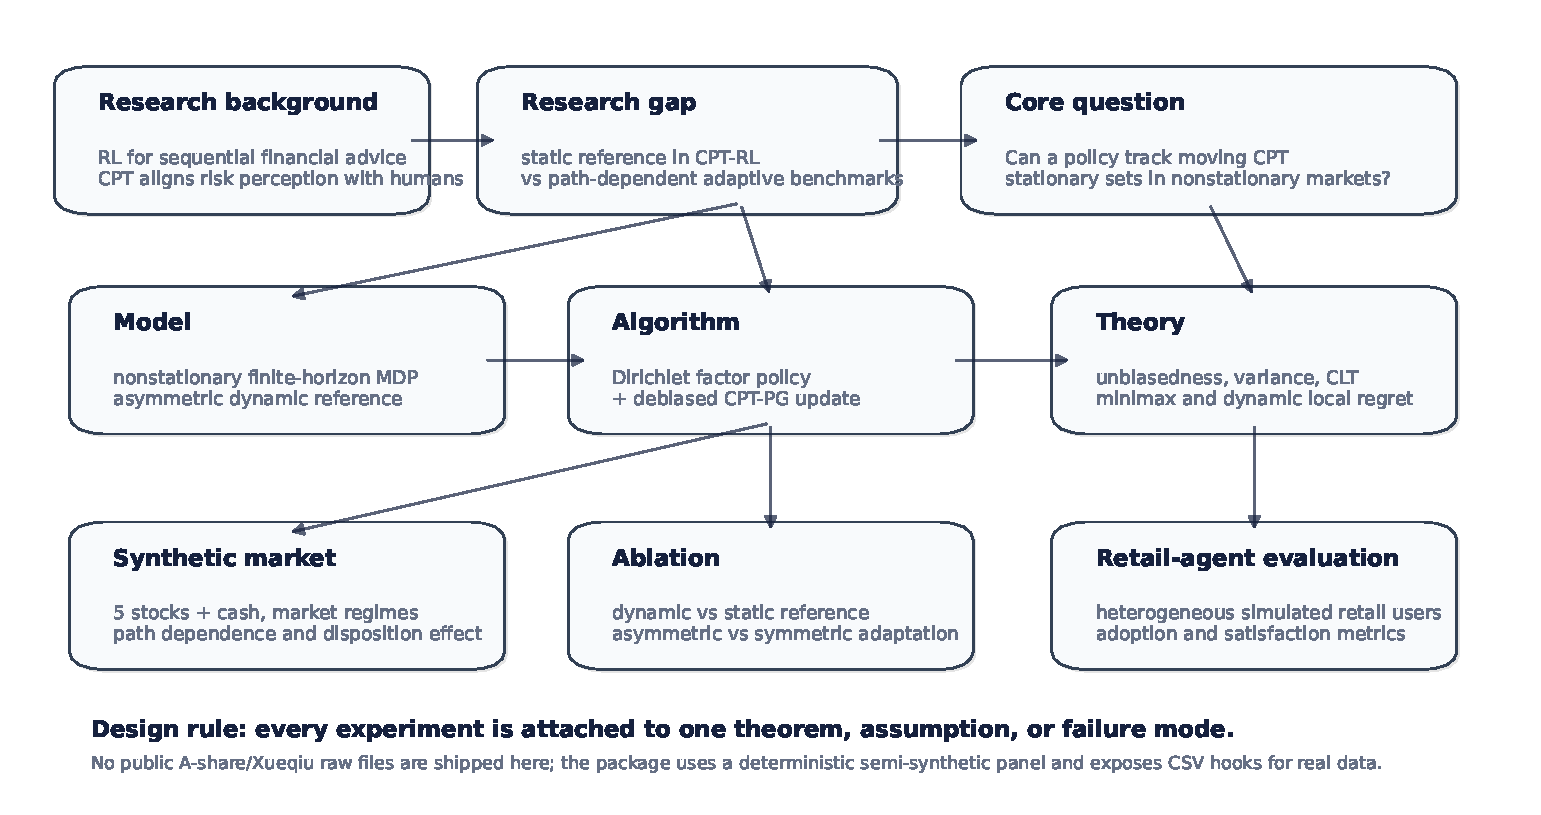
\includegraphics[width=\textwidth]{fig_opening_report_alignment_final.pdf}
\caption{Project map aligned with the opening-report logic.  The pipeline starts from human-facing RL, isolates the static-reference gap in \CPT-RL, defines dynamic-reference \CPT-PG, then links estimator theory, dynamic regret, semi-synthetic market validation, ablation, and heterogeneous retail-agent evaluation.}
\label{fig:report-map}
\end{figure}

\subsection{Behavioral mechanism: path dependence and disposition effect}

\begin{figure}[t]
\centering
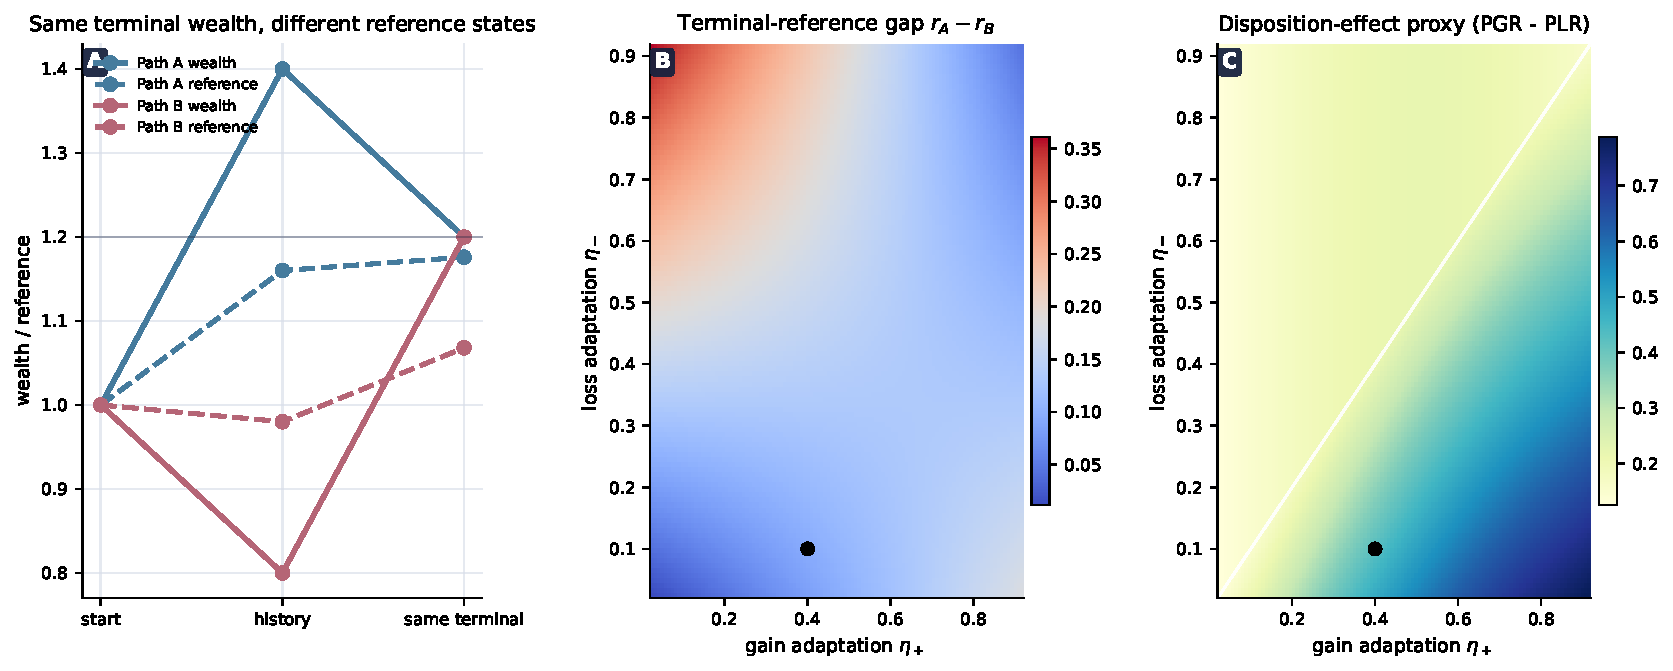
\includegraphics[width=\textwidth]{fig_path_disposition_final.pdf}
\caption{Behavioral mechanism.  Panel A shows two paths with identical terminal wealth but different terminal references.  Panel B visualizes the terminal-reference gap in \Cref{prop:path-dependence}.  Panel C reports a disposition-effect proxy, illustrating how $\etaP>\etaM$ strengthens the gap between selling gains and selling losses.}
\label{fig:path-disposition}
\end{figure}

\subsection{Estimator diagnostics: unbiasedness, variance, CLT, minimax rate}

\begin{figure}[t]
\centering
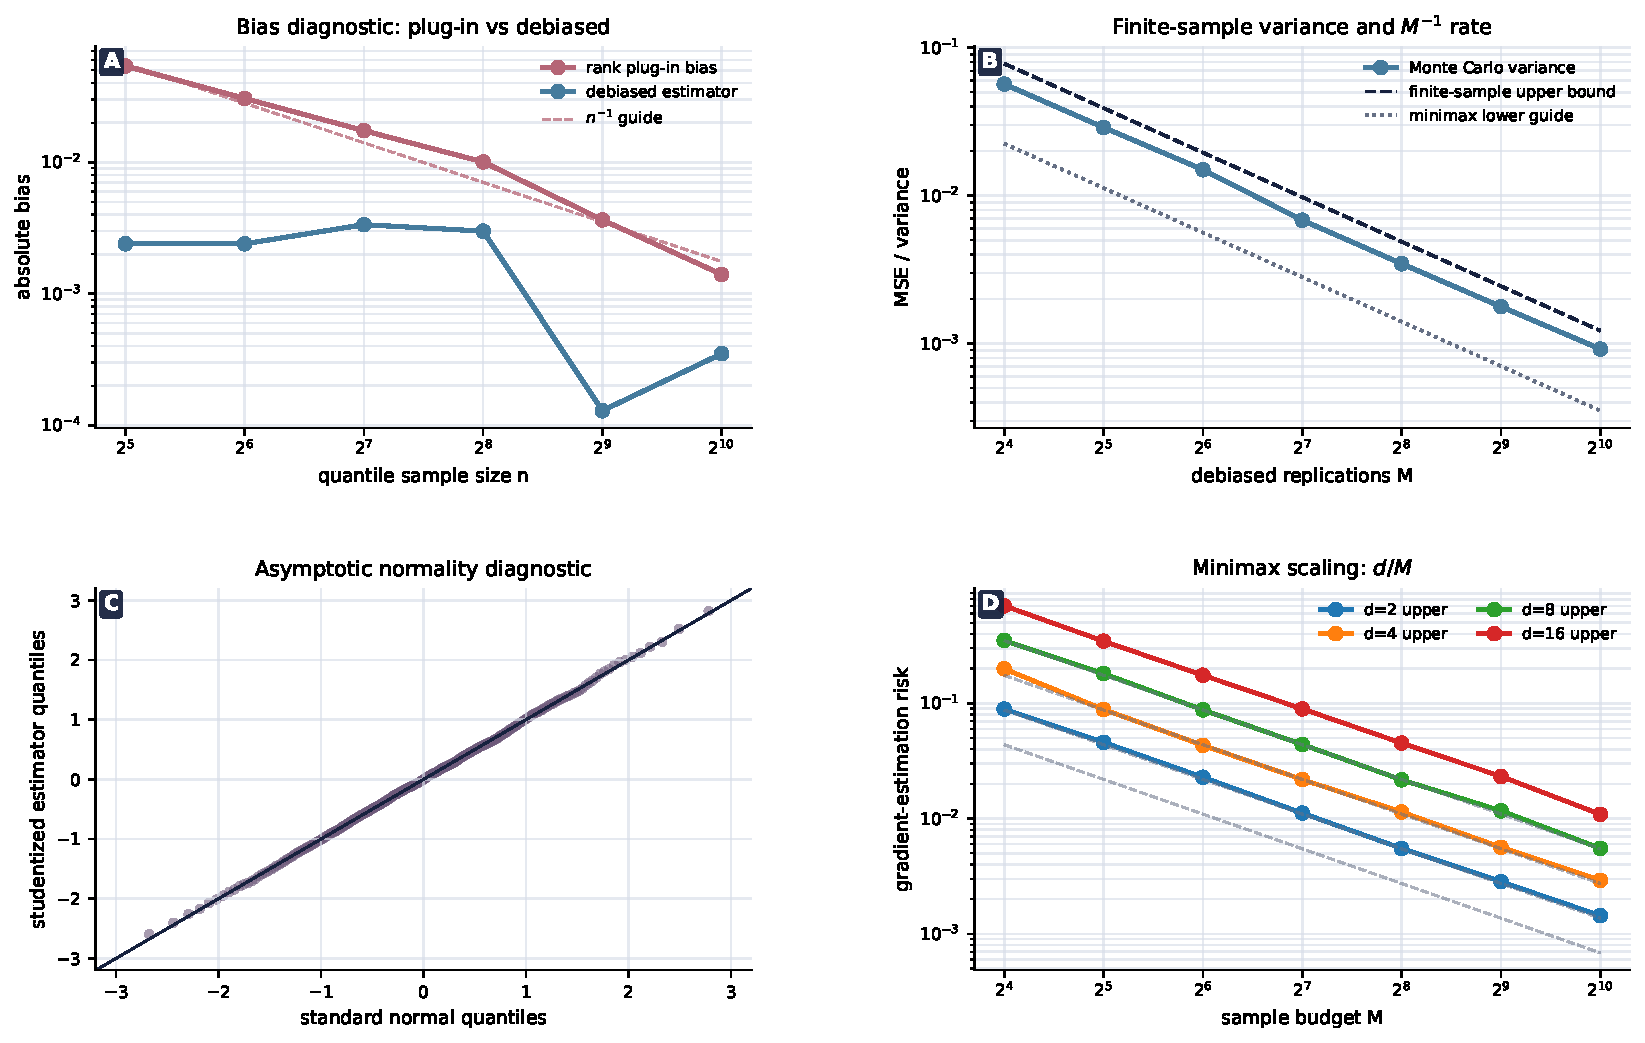
\includegraphics[width=\textwidth]{fig_estimator_theory_final.pdf}
\caption{Estimator-theory diagnostics.  Panel A shows the rank plug-in bias and the centered debiased estimator.  Panel B validates the finite-sample $M^{-1}$ variance scaling and displays a minimax lower guide.  Panel C gives a studentized normal-quantile diagnostic.  Panel D illustrates the $d/M$ minimax scaling.}
\label{fig:estimator-theory}
\end{figure}

\subsection{Synthetic nonstationary market tracking}

\begin{figure}[t]
\centering
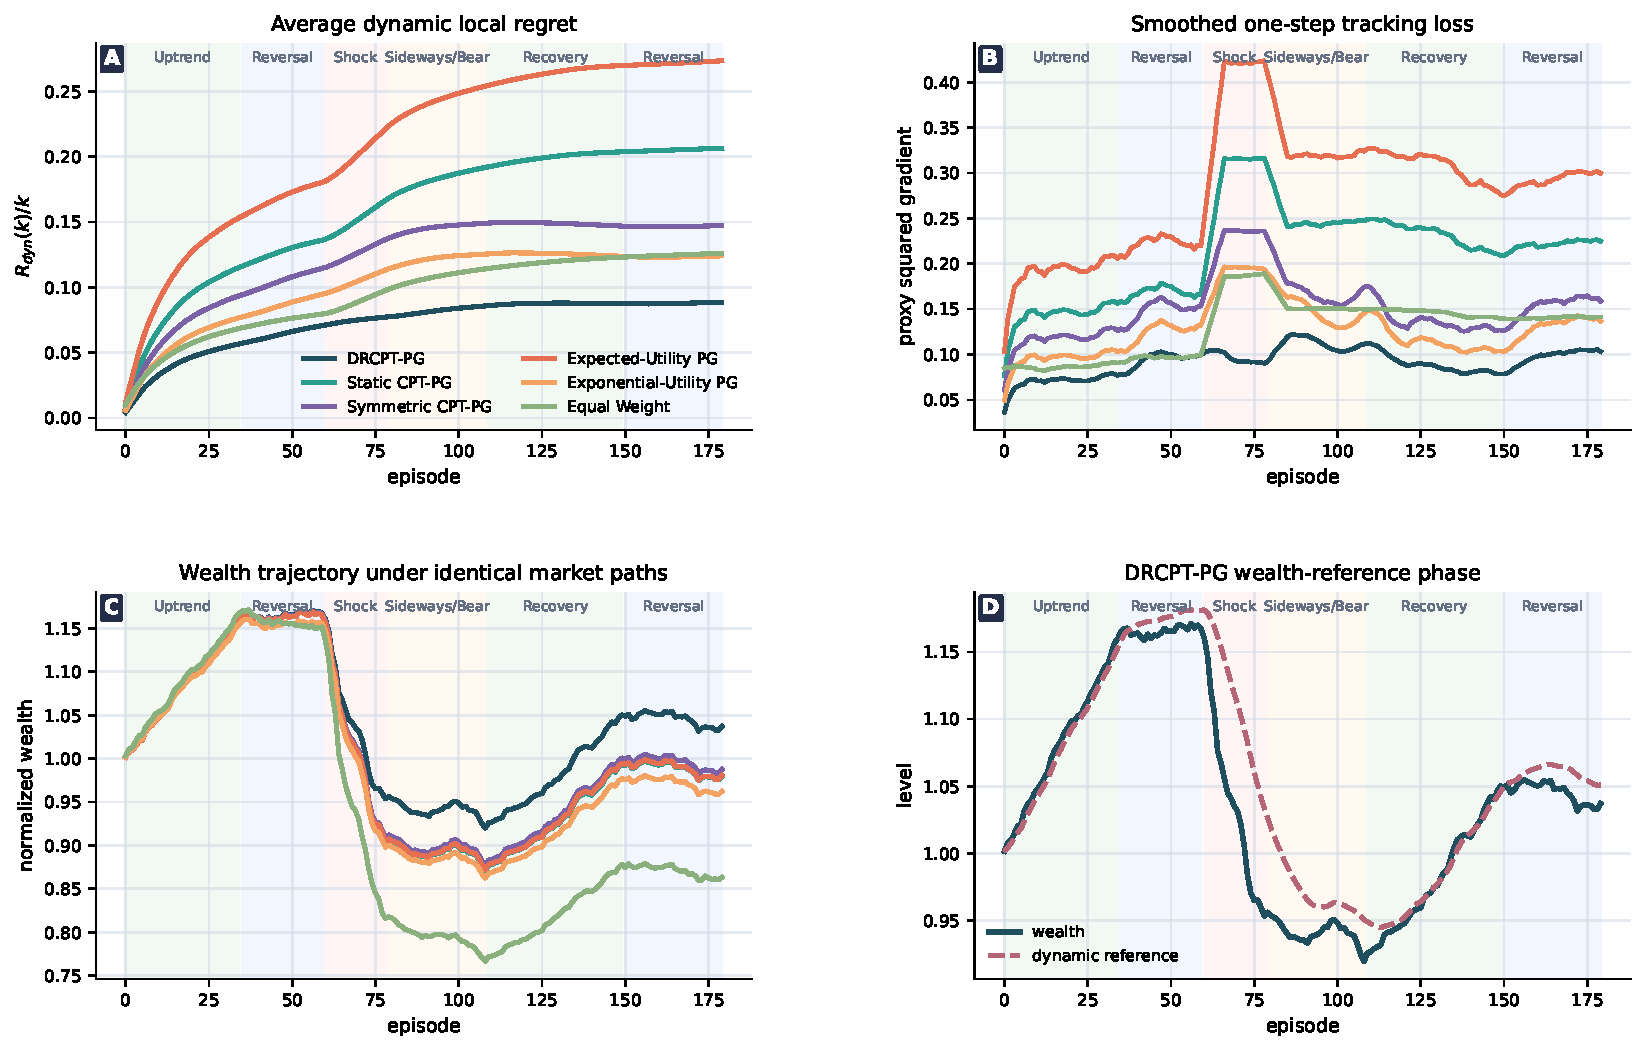
\includegraphics[width=\textwidth]{fig_tracking_regret_final.pdf}
\caption{Dynamic tracking in a controlled nonstationary market.  Panels A and B show that \DRCPTPG has lower average dynamic local regret and lower one-step tracking loss after the shock than static-reference and expected-utility baselines.  Panel C compares wealth trajectories under identical market paths.  Panel D shows the endogenous wealth-reference dynamics for \DRCPTPG.}
\label{fig:tracking}
\end{figure}

\begin{figure}[t]
\centering
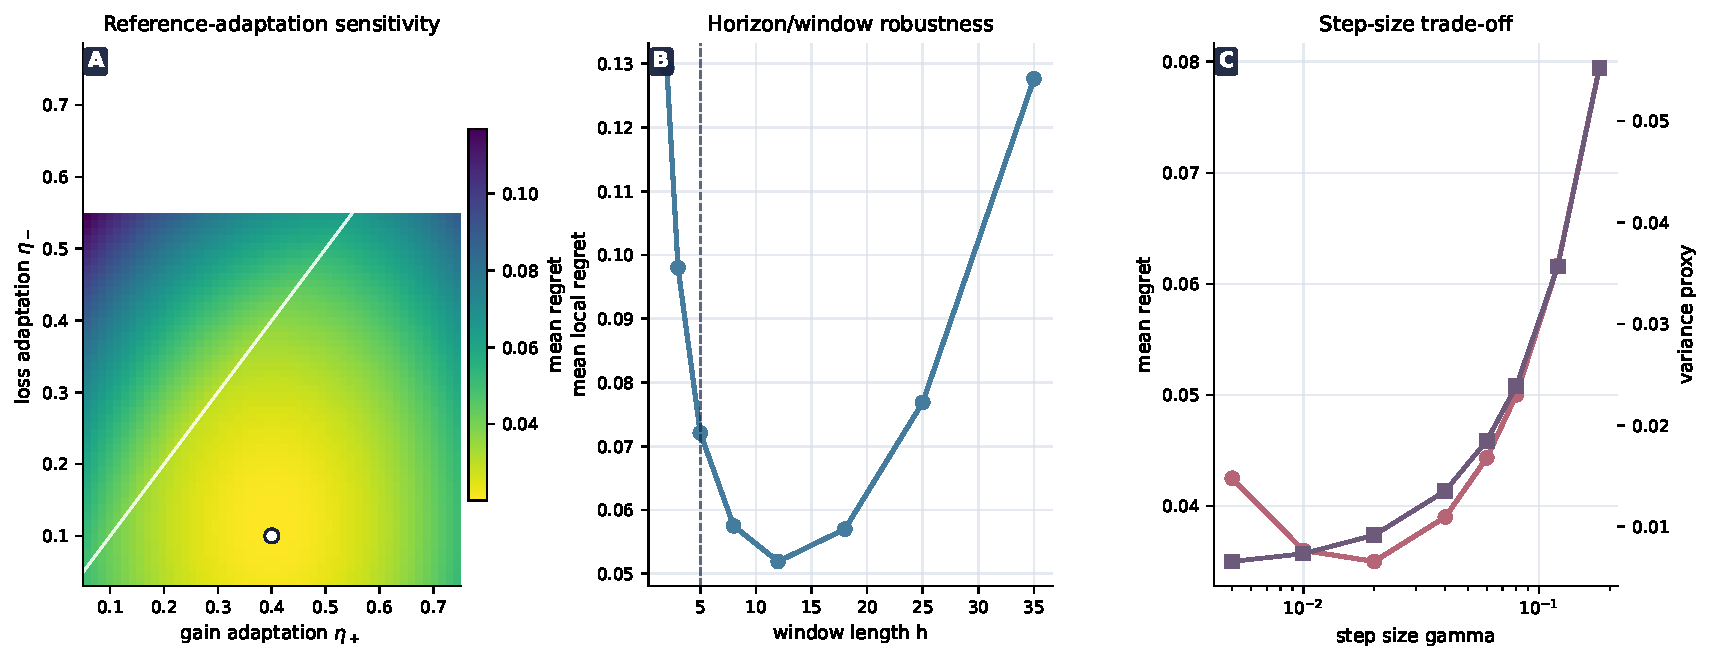
\includegraphics[width=\textwidth]{fig_ablation_sensitivity_final.pdf}
\caption{Ablation and sensitivity.  Panel A varies $(\etaP,\etaM)$ and shows that asymmetric but not overly aggressive adaptation minimizes tracking regret.  Panel B varies the horizon/window length.  Panel C varies the step size and displays the regret-variance trade-off predicted by \Cref{thm:dynamic-regret}.}
\label{fig:ablation}
\end{figure}

\subsection{Semi-synthetic A-share-style replay}

The semi-synthetic panel contains five stock-like assets plus cash, observable factors, and regimes labeled uptrend, reversal, shock, sideways/bear, recovery, and reversal.  This corresponds to the report's design logic of using real-style factors while controlling the market regime and shock mechanism.

\begin{figure}[t]
\centering
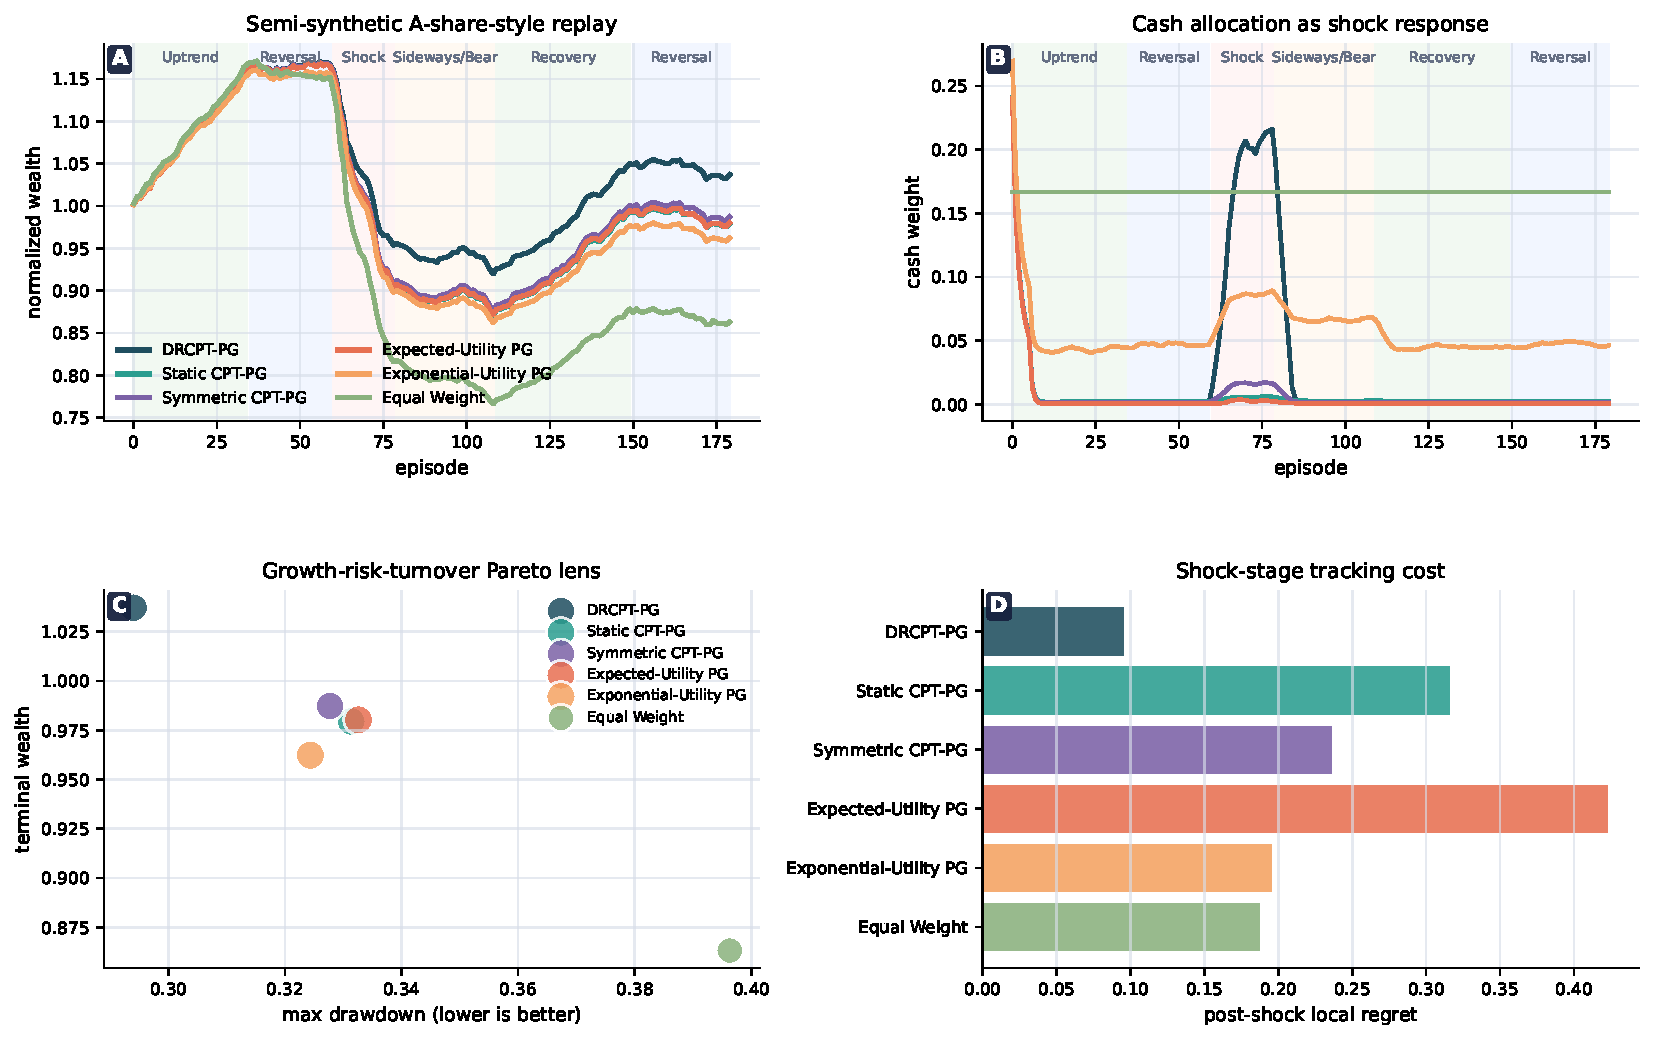
\includegraphics[width=\textwidth]{fig_ashare_semisynthetic_final.pdf}
\caption{Semi-synthetic A-share-style portfolio replay.  Panel A compares wealth trajectories.  Panel B shows cash allocation as a shock-response mechanism.  Panel C places methods on a growth-risk-turnover lens.  Panel D reports post-shock tracking cost, where \DRCPTPG has the smallest local regret among the plotted policy-gradient baselines.}
\label{fig:ashare}
\end{figure}

\subsection{Heterogeneous retail-agent evaluation}

The retail-agent evaluation simulates five investor types: loss-averse, trend-chasing, drawdown-averse, turnover-sensitive, and balanced.  Each type scores recommendations from five advisor agents: dynamic-reference \CPTPG, static-reference \CPTPG, symmetric-reference \CPTPG, expected-utility PG, and exponential-utility PG.  The metrics are satisfaction and adoption probability.

\begin{figure}[t]
\centering
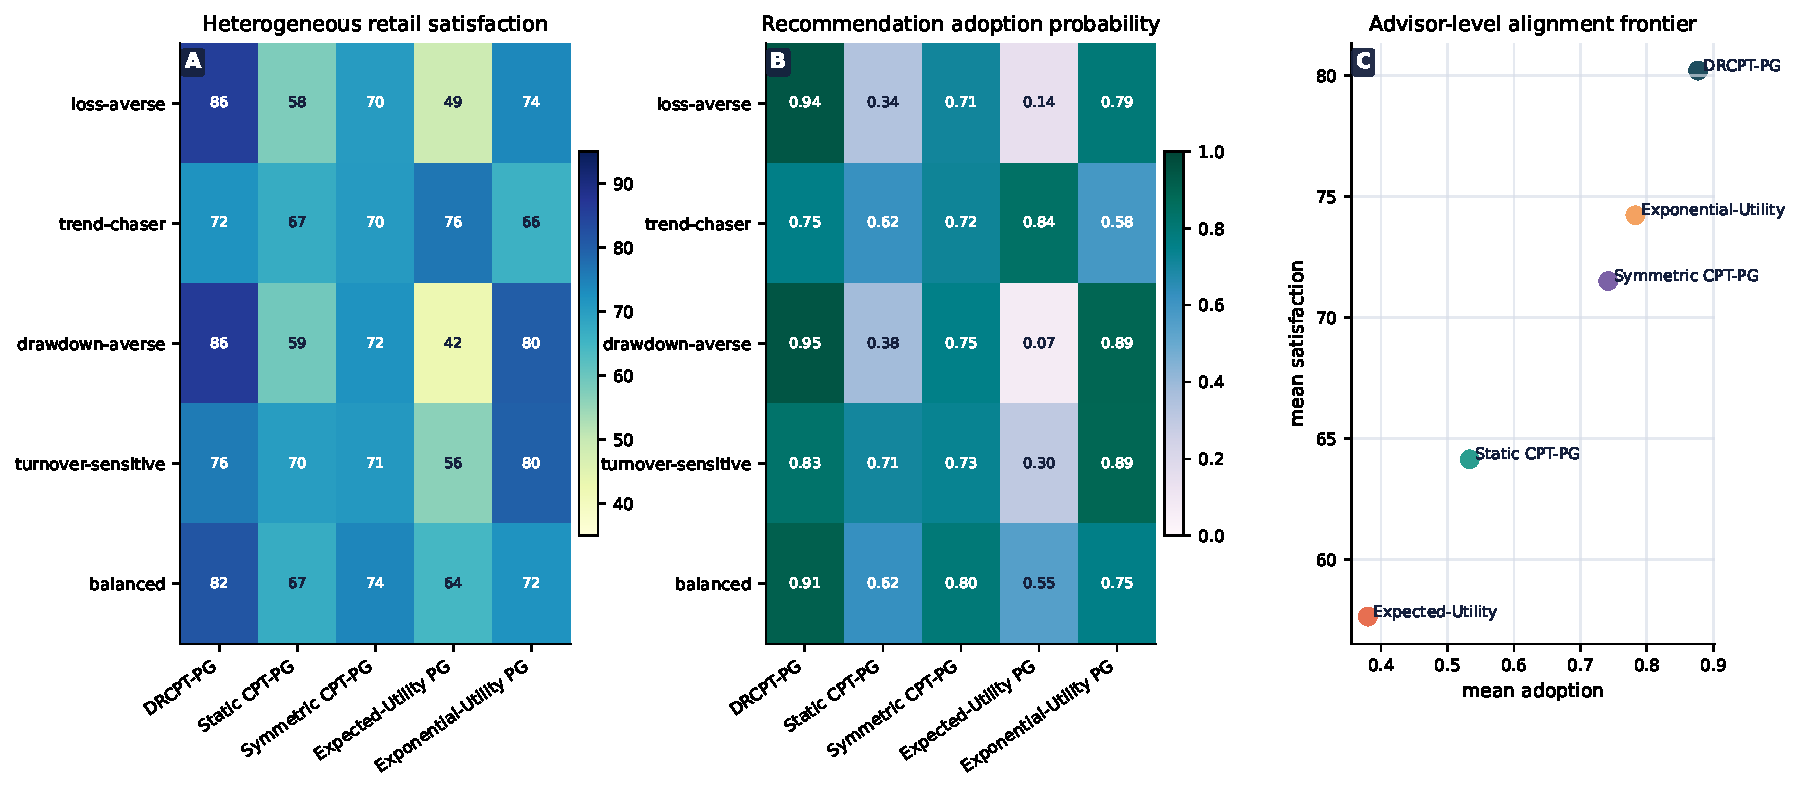
\includegraphics[width=\textwidth]{fig_retail_multiagent_final.pdf}
\caption{Heterogeneous retail-agent evaluation.  Panel A reports satisfaction by investor type and advisor.  Panel B reports adoption probability.  Panel C summarizes the advisor-level alignment frontier.  The experiment tests whether dynamic-reference \CPTPG is more acceptable to behaviorally heterogeneous users, rather than merely wealth-maximizing.}
\label{fig:retail}
\end{figure}

\FloatBarrier
\section{Discussion}\label{sec:discussion}

This paper studies the point where behavioral decision theory changes the mathematical target of reinforcement learning.  If the reference point is fixed, \CPTPG is a nonconvex but stationary policy-gradient problem.  If the reference point adapts along the wealth path, the agent must track a moving stationary set.  The main theorem turns this intuition into a bound: tracking error is governed by sample size, step size, market drift, and reference drift.

The limitations are important.  First, the theory is local and first-order; it does not promise global optimization of a nonconvex \CPT objective.  Second, the reference-update law is parametric.  In a deployed advisor, $\etaP$ and $\etaM$ should be calibrated to user-level behavior and stress-tested.  Third, public price data do not reveal latent psychological reference points.  The semi-synthetic and simulated retail experiments validate mechanisms, not unobserved human satisfaction.  Fourth, the regularization parameter $\eps$ is part of the estimable objective and must be reported.

These boundaries are also the research agenda.  Future work should combine dynamic-reference \CPTPG with user-specific calibration, off-policy evaluation for behavioral objectives, real retail adoption data, and reset mechanisms for large structural breaks.  More broadly, human-aligned reinforcement learning should model not only what a user values, but also how the user's evaluation state evolves through interaction.

\clearpage
\bibliographystyle{plainnat}
\bibliography{references}

\clearpage
\appendix

\section{Notation and Reproducibility Convention}\label{app:notation}

All theoretical statements are conditional on the information $\cF_k$ available at the start of episode $k$.  The real execution path updates the actual wealth and reference point.  The learning layer uses simulated or bootstrapped horizon-$h$ trajectories from the episode-start state to estimate the \CPT gradient.

\begin{table}[h]
\centering
\caption{Main notation.}
\begin{tabular}{ll}
\toprule
Symbol & Meaning \\
\midrule
$X_u$ & normalized wealth after date $u$ \\
$r_u$ & psychological reference point \\
$\etaP,\etaM$ & reference adaptation rates after gains and losses \\
$Y_k=X_k-r_{k,h}$ & terminal relative outcome in episode $k$ \\
$J_k(\theta,r_k)$ & regularized dynamic-reference \CPT objective \\
$\pi_\theta$ & Dirichlet portfolio policy \\
$G_{k,\theta}(\tau)$ & trajectory score function \\
$g_k$ & true \CPT policy gradient at $\theta_k$ \\
$\widehat g_k^{\pl}$ & rank plug-in \CPT gradient estimator \\
$\widehat g_k^{\db}$ & multilevel debiased \CPT gradient estimator \\
$\delta_k$ & horizon-$h$ market drift budget \\
$\Sta_k$ & first-order stationary set of $J_k$ \\
$\Reg_{\rho,w}(K)$ & discounted-window dynamic local regret \\
\bottomrule
\end{tabular}
\end{table}

\section{Proofs for the Reference Mechanism}\label{app:reference-proofs}

\subsection{Proof of \Cref{prop:path-dependence}}
\begin{proof}
For path $A$, the first step is a gain from $r_0$ to $H$, so the interim reference is
\[
 r_A^{(1)}=(1-\etaP)r_0+\etaP H.
\]
By assumption, the second step from $H$ to $C$ is below this interim reference; hence the loss-side update gives
\[
 r_A=(1-\etaM)r_A^{(1)}+\etaM C
 =(1-\etaM)\{(1-\etaP)r_0+\etaP H\}+\etaM C.
\]
For path $B$, the first step is a loss, so
\[
 r_B^{(1)}=(1-\etaM)r_0+\etaM L.
\]
The second step to $C$ is above $r_B^{(1)}$, so
\[
 r_B=(1-\etaP)r_B^{(1)}+\etaP C
 =(1-\etaP)\{(1-\etaM)r_0+\etaM L\}+\etaP C.
\]
Subtracting the two displays cancels the coefficient of $r_0$ and gives \eqref{eq:path-diff}.  If $r_A\ne r_B$, the relative outcomes $C-r_A$ and $C-r_B$ differ.  The regularized gain and loss value functions are monotone, and the probability weights are monotone; hence the induced \CPT inputs differ except in degenerate flat regions excluded by the smoothing construction.
\end{proof}

\section{Proofs for the CPT Gradient and Estimator}\label{app:estimator-proofs}

\subsection{Proof of \Cref{thm:gradient-identity}}
\begin{proof}
We prove the gain part; the loss part is identical with a minus sign.  Let
\[
 J_k^+(\theta)=\int_0^{B_v} w_+^\eps(S^+_{k,\theta}(z))\,dz.
\]
By Assumption \ref{ass:smooth-cpt}, $\dot w_+^\eps$ is bounded.  By differentiability in quadratic mean and the score identity,
\[
 \nabla_\theta S^+_{k,\theta}(z)
 =\nabla_\theta \E_{k,\theta}\1[v_+(Y_k)>z]
 =\E_{k,\theta}\{\1[v_+(Y_k)>z]G_{k,\theta}(\tau)\}.
\]
Dominated convergence is justified by Assumption \ref{ass:bounded}.  Therefore
\begin{align*}
 \nabla_\theta J_k^+(\theta)
 &=\int_0^{B_v}\dot w_+^\eps(S^+_{k,\theta}(z))
 \E\{\1[v_+(Y_k)>z]G_{k,\theta}(\tau)\}\,dz\\
 &=\E\left[\left\{\int_0^{B_v}\dot w_+^\eps(S^+_{k,\theta}(z))\1[v_+(Y_k)>z]dz\right\}G_{k,\theta}(\tau)\right].
\end{align*}
Since $\E G_{k,\theta}(\tau)=0$, subtracting $S^+_{k,\theta}(z)$ inside the braces does not change the expectation.  Repeating the argument for the loss integral and subtracting proves \eqref{eq:gradient-identity}.
\end{proof}

\subsection{Proof of \Cref{prop:debias}}
\begin{proof}
For the plug-in estimator, write the empirical survival functions as $\widehat S_n^\pm$.  Because $\dot w_\pm^\eps$ is continuously differentiable with bounded derivative,
\[
 \dot w_\pm^\eps(\widehat S_n^\pm(z))-\dot w_\pm^\eps(S^\pm(z))
 =\ddot w_\pm^\eps(S^\pm(z))(\widehat S_n^\pm(z)-S^\pm(z))+R_n(z),
\]
where $\abs{R_n(z)}\le C\abs{\widehat S_n^\pm(z)-S^\pm(z)}^2$.  Cross-fitting makes the rank sample independent of the score sample.  The first-order empirical-survival error has mean zero, while the second-order term has expectation $O(n^{-1})$ uniformly in $z$ by the Dvoretzky-Kiefer-Wolfowitz inequality and boundedness.  Multiplication by the bounded score and integration over $[0,B_v]$ yield the $C_{\rm b}/n$ term.  The $C_{\rm d}\delta_k$ term follows from the bounded-Lipschitz drift assumption and the Lipschitzness of the regularized score kernel.

For the debiased estimator, define $\Delta_{k,0}=T_{k,0}$ and, for $\ell\ge1$,
\[
 \Delta_{k,\ell}=T_{k,\ell}-{1\over2}(T_{k,\ell-1}^{(1)}+T_{k,\ell-1}^{(2)}).
\]
Then
\[
 \E(\Delta_{k,0}\mid\cF_k)=\mu_{k,0},\qquad
 \E(\Delta_{k,\ell}\mid\cF_k)=\mu_{k,\ell}-\mu_{k,\ell-1},\quad \ell\ge1.
\]
Assumption \ref{ass:mlmc} implies $\mu_{k,\ell}\to g_k$.  Hence the telescoping series is absolutely convergent and
\[
 \sum_{\ell=0}^{\infty}\E(\Delta_{k,\ell}\mid\cF_k)=g_k.
\]
If $L$ is independent of the trajectory draws with $\Pp(L=\ell)=p_\ell$, then
\[
 \E(Z_k^{\db}\mid\cF_k)
 =\sum_{\ell=0}^{\infty}p_\ell {\E(\Delta_{k,\ell}\mid\cF_k)\over p_\ell}=g_k.
\]
For the second moment,
\[
 \E\norm{Z_k^{\db}}_2^2
 =\sum_{\ell=0}^{\infty}{\E\norm{\Delta_{k,\ell}}_2^2\over p_\ell}
 \le C\sum_{\ell=0}^{\infty}{2^{-2\ell}\over 2^{-a\ell}}<\infty
\]
because $a<2$.  The expected cost is bounded by
\[
 C\sum_{\ell=0}^{\infty}p_\ell 2^\ell
 \le C\sum_{\ell=0}^{\infty}2^{-(a-1)\ell}<\infty
\]
because $a>1$.  If the sum is truncated at $L_{\max}$, the remaining bias is
\[
 \norm{\sum_{\ell>L_{\max}}\E\Delta_{k,\ell}}_2
 =\norm{g_k-\mu_{k,L_{\max}}}_2\le A_{\rm ml}2^{-L_{\max}}.
\]
\end{proof}

\subsection{Proof of \Cref{thm:variance}}
\begin{proof}
Unbiasedness follows immediately from \Cref{prop:debias}.  Since the $M$ debiased replications are conditionally independent,
\[
 \tr\Var(\widehat g_{k,M}^{\db}\mid\cF_k)
 ={1\over M}\tr\Var(Z_k^{\db}\mid\cF_k)
 \le {1\over M}\E\norm{Z_k^{\db}}_2^2
 \le {C_{\db}\over M}.
\]
For the plug-in estimator, decompose
\[
 \widehat g_{k,n,m}^{\pl}-g_k
 =\{\widehat g_{k,n,m}^{\pl}-\E(\widehat g_{k,n,m}^{\pl}\mid\widehat S_n,\cF_k)\}
 +\{\E(\widehat g_{k,n,m}^{\pl}\mid\widehat S_n,\cF_k)-g_k\}.
\]
The first term is a mean of $m$ independent bounded score-kernel variables, so its second moment is $O(m^{-1})$.  The second term is controlled by the empirical-survival error and the drift error; the same Taylor and DKW argument used in \Cref{prop:debias} gives $O(n^{-1})+O(\delta_k^2)+O(n^{-2})$ after squaring the bias.  Combining the terms proves \eqref{eq:plugin-mse}.
\end{proof}

\subsection{Proof of \Cref{thm:clt}}
\begin{proof}
Conditional on $\cF_k$, the vectors $Z_{k,1}^{\db},\ldots,Z_{k,M}^{\db}$ are independent and identically distributed with mean $g_k$, covariance $\Sigma_k$, and a finite $(2+\xi)$ moment.  The multivariate Lindeberg-Feller central limit theorem gives
\[
 \sqrt{M}\,\Sigma_k^{-1/2}(\widehat g_{k,M}^{\db}-g_k)\rightsquigarrow N(0,I_d).
\]
For fixed $d$, the empirical covariance $\widehat\Sigma_k$ is consistent by the law of large numbers for matrices under the same moment condition.  Slutsky's theorem yields the studentized convergence.
\end{proof}

\section{Proofs for Stationary-Set Drift and Dynamic Regret}\label{app:regret-proofs}

\subsection{Proof of \Cref{lem:set-drift}}
\begin{proof}
Fix $\theta\in\Sta_k$.  Then $\nabla J_k(\theta,r_k)=0$.  By \eqref{eq:gradient-drift},
\[
 \norm{\nabla J_{k+1}(\theta,r_{k+1})}_2
 \le L_D\{\delta_k+\abs{r_{k+1}-r_k}\}.
\]
Applying the error-bound Assumption \ref{ass:error-bound} to $J_{k+1}$ gives
\[
 \dist(\theta,\Sta_{k+1})
 \le \kappa L_D\{\delta_k+\abs{r_{k+1}-r_k}\}.
\]
Taking the supremum over $\theta\in\Sta_k$ yields one directed Hausdorff bound.  Repeating the same argument with $k$ and $k+1$ interchanged gives the other directed bound after increasing $L_D$ if necessary.  Taking the maximum gives \eqref{eq:set-drift}.
\end{proof}

\subsection{Projected ascent inequality}
\begin{lemma}[One-step projected ascent]\label{lem:projected-ascent}
Under Assumption \ref{ass:smooth-cpt}, the projected update $\theta_{k+1}=\Pi_{\ThetaSet}(\theta_k+\gamma d_k)$ satisfies
\begin{equation}\label{eq:projected-ascent}
 J_k(\theta_{k+1},r_k)
 \ge J_k(\theta_k,r_k)+\gamma\ip{g_k,d_k}-C_P\gamma^2\norm{d_k}_2^2
\end{equation}
for a constant $C_P<\infty$ depending only on the local smoothness and the compact convex set $\ThetaSet$.
\end{lemma}
\begin{proof}
If no projection occurs, \eqref{eq:projected-ascent} is the standard lower quadratic bound for an $L$-smooth function being maximized:
\[
 J_k(\theta_k+\gamma d_k,r_k)
 \ge J_k(\theta_k,r_k)+\gamma\ip{g_k,d_k}-{L\gamma^2\over2}\norm{d_k}_2^2.
\]
If projection occurs, nonexpansiveness of Euclidean projection and compactness of $\ThetaSet$ imply that the projected and unprojected points differ by at most $O(\gamma\norm{d_k})$ on the local tangent cone.  Smoothness then bounds the additional objective loss by $C\gamma^2\norm{d_k}_2^2$.  Absorbing constants gives the claim.
\end{proof}

\subsection{Proof of \Cref{thm:dynamic-regret}}
\begin{proof}
By \Cref{lem:projected-ascent} and Assumption \ref{ass:alignment},
\begin{align}
 c_d\gamma\E\norm{g_k}_2^2
 &\le \E\{J_k(\theta_{k+1},r_k)-J_k(\theta_k,r_k)\}
 +C_P\gamma^2D_d^2
 +c_e\gamma\E\norm{\widehat g_k^{\db}-g_k}_2^2.\label{eq:one-step}
\end{align}
Using the value-drift inequality \eqref{eq:value-drift},
\[
 J_k(\theta_{k+1},r_k)
 \le J_{k+1}(\theta_{k+1},r_{k+1})
 +L_J\{\delta_k+\abs{r_{k+1}-r_k}\}.
\]
Substituting into \eqref{eq:one-step} and summing over $k=1,\ldots,K$ gives
\begin{align*}
 c_d\gamma\sum_{k=1}^{K}\E\norm{g_k}_2^2
 &\le \E\{J_{K+1}(\theta_{K+1},r_{K+1})-J_1(\theta_1,r_1)\}
 +C\gamma^2K \\
 &\quad +c_e\gamma\sum_{k=1}^{K}\E\norm{\widehat g_k^{\db}-g_k}_2^2
 +L_J\sum_{k=1}^{K}\{\delta_k+\abs{r_{k+1}-r_k}\}.
\end{align*}
The endpoint difference is bounded by Assumption \ref{ass:bounded}.  By \Cref{thm:variance},
\[
 \E\norm{\widehat g_k^{\db}-g_k}_2^2\le {C_{\db}\over M_k}.
\]
If the finite-horizon simulation law itself drifts within the episode, the regularized score-kernel Lipschitz condition contributes the $C_3\sum\delta_k^2$ term.  Dividing by $K\gamma$ gives a bound for $K^{-1}\sum_k\E\norm{g_k}_2^2$.

It remains to pass from raw gradients to the smoothed local regret.  By Jensen's inequality,
\[
 \norm{\bar g_k}_2^2
 \le {1\over A_k}\sum_{j=0}^{\min\{w-1,k-1\}}\rho^j\norm{g_{k-j}}_2^2.
\]
Each $\norm{g_i}_2^2$ appears in at most $w$ future windows with total coefficient bounded by $w$.  Hence
\[
 \Reg_{\rho,w}(K)\le w\sum_{k=1}^{K}\norm{g_k}_2^2.
\]
Absorbing the fixed window factor into the constants proves \eqref{eq:main-bound}.  A truncated debiased estimator has squared bias $O(2^{-2L_{k,\max}})$ by \Cref{prop:debias}, which adds the final stated term.
\end{proof}

\subsection{Proof of \Cref{cor:static}}
\begin{proof}
When the market and reference are fixed, $\delta_k=0$ and $r_{k+1}=r_k=r$.  The objectives are all the same function $J(\cdot,r)$.  If $M_k\to\infty$, the estimator-variance term vanishes in Cesaro average.  \Cref{thm:dynamic-regret} therefore yields
\[
 \limsup_{K\to\infty}{1\over K}\sum_{k=1}^{K}\E\norm{\nabla J(\theta_k,r)}_2^2\le C\gamma.
\]
A decreasing step-size proof follows the same telescoping argument with $\sum_k\gamma_k=\infty$ and $\sum_k\gamma_k^2<\infty$.
\end{proof}

\subsection{Proof of \Cref{cor:set-tracking}}
\begin{proof}
Assumption \ref{ass:error-bound} gives
\[
 \dist^2(\theta_k,\Sta_k)\le \kappa^2\norm{\nabla J_k(\theta_k,r_k)}_2^2=\kappa^2\norm{g_k}_2^2.
\]
Averaging over $k$ and taking expectations proves \eqref{eq:set-tracking}.  The dynamic-regret theorem controls the average gradient norm up to fixed smoothing-window constants.
\end{proof}

\section{Proof of the Minimax Lower Bound}\label{app:minimax-proof}

\subsection{Proof of \Cref{thm:minimax}}
\begin{proof}
It is enough to prove the result for a subclass.  Let $v\in\{-1,1\}^d$ and define a product distribution $P_v$ on $Z\in\{-B_0,B_0\}^d$ by
\[
 \Pp_v(Z_j=B_0)={1+\alpha v_j\over2},
 \qquad
 \Pp_v(Z_j=-B_0)={1-\alpha v_j\over2},
\]
where $B_0\asymp \sigma$ and $0<\alpha<1/2$.  The mean is
\[
 g(P_v)=B_0\alpha v.
\]
For two vertices $v$ and $v'$ differing only in coordinate $j$, the Kullback-Leibler divergence between one observation from $P_v$ and one from $P_{v'}$ is at most $C\alpha^2$.  Therefore the divergence between $M$ observations is at most $CM\alpha^2$.  Choose $\alpha=c_0M^{-1/2}$ with $c_0$ small enough so that this divergence is bounded by a universal constant.

By Assouad's lemma,
\[
 \inf_{\widehat g}\sup_{v\in\{-1,1\}^d}
 \E_v\norm{\widehat g-g(P_v)}_2^2
 \ge c\,d(B_0\alpha)^2
 \ge c' {d\sigma^2\over M}.
\]
The distributions are supported in $[-B_Z,B_Z]^d$ when $B_0\le B_Z$, and their coordinate variances are of order $\sigma^2$.  Since the subclass is contained in $\mathfrak P(d,B_Z,\sigma)$, the lower bound holds for the whole class.
\end{proof}

\section{Experimental Reproducibility Details}\label{app:experiments}

The project is organized as follows.
\begin{center}
\small
\begin{tabularx}{\textwidth}{>{\raggedright\arraybackslash}p{0.48\textwidth}X}
\toprule
Path & Purpose \\
\midrule
\texttt{main.tex} & manuscript source \\
\texttt{references.bib} & bibliography \\
\texttt{figures/} & exported PDF, PNG, and SVG figures \\
\texttt{experiments/generate\_experiments.py} & deterministic experiment generator \\
\texttt{data/ashare\_panel.csv} & semi-synthetic market panel (full file name documented in the data README) \\
\texttt{data/README\_data.md} & instructions for replacing shipped data with local Tushare/Xueqiu CSV files \\
\texttt{experiments/results/} & numerical summaries used in figures and tables \\
\bottomrule
\end{tabularx}
\end{center}
The script can be rerun with
\begin{center}
\texttt{python experiments/generate\_experiments.py}.
\end{center}
For deterministic linear algebra on multi-core machines, one may set
\begin{center}
\texttt{OPENBLAS\_NUM\_THREADS=1 OMP\_NUM\_THREADS=1 MKL\_NUM\_THREADS=1}.
\end{center}
The shipped A-share and retail-agent results are semi-synthetic.  They are designed to validate the theoretical mechanism under controlled regimes and do not claim to be raw Tushare or Xueqiu measurements.

\end{document}
